\documentclass[sigconf,review,anonymous,screen]{acmart}



%%
%% \BibTeX command to typeset BibTeX logo in the docs
\AtBeginDocument{%
	\providecommand\BibTeX{{%
			\normalfont B\kern-0.5em{\scshape i\kern-0.25em b}\kern-0.8em\TeX}}}

%% Rights management information.  This information is sent to you
%% when you complete the rights form.  These commands have SAMPLE
%% values in them; it is your responsibility as an author to replace
%% the commands and values with those provided to you when you
%% complete the rights form.
\setcopyright{acmcopyright}
\copyrightyear{2018}
\acmYear{2018}
\acmDOI{10.1145/1122445.1122456}

%% These commands are for a PROCEEDINGS abstract or paper.
\acmConference[ICSE 2022]{The 44th International Conference on Software Engineering}{May 21–29, 2022}{Pittsburgh, PA, USA}
\acmBooktitle{ICSE '22: Proceedings of the 44th International Conference on Software Engineering,
	May 21–29, 2022, Pittsburgh, PA, USA}
\acmPrice{15.00}
\acmISBN{978-1-4503-XXXX-X/18/06}


%%
%% Submission ID.
%% Use this when submitting an article to a sponsored event. You'll
%% receive a unique submission ID from the organizers
%% of the event, and this ID should be used as the parameter to this command.
%%\acmSubmissionID{123-A56-BU3}

%%
%% The majority of ACM publications use numbered citations and
%% references.  The command \citestyle{authoryear} switches to the
%% "author year" style.
%%
%% If you are preparing content for an event
%% sponsored by ACM SIGGRAPH, you must use the "author year" style of
%% citations and references.
%% Uncommenting
%% the next command will enable that style.
%%\citestyle{acmauthoryear}

%%
%% end of the preamble, start of the body of the document source.


\usepackage{blindtext}

\usepackage{listings}

\usepackage{pifont}
\newcommand{\xmark}{\ding{55}}

\usepackage{xcolor}
\usepackage{tabularx}

% general imports
%\usepackage{amsmath,amssymb,amsfonts}

\usepackage{algorithmic}
\usepackage{graphicx}


% layout and formatting
\usepackage{microtype}

\usepackage{subcaption}

% configure hyperlinks 
\usepackage{hyperref}
\hypersetup{
	colorlinks,
	linkcolor={green!90!white},
	citecolor={blue},
	urlcolor={green!80!black}
}

% nice monospace font
%\usepackage{sourcecodepro}

%\usepackage{enumitem}


\usepackage{pdfcomment}

\usepackage{makecell}

\renewcommand\theadalign{bc}
\renewcommand\theadfont{\bfseries}
\renewcommand\theadgape{\Gape[0pt]}
\renewcommand\cellgape{\Gape[0pt]}

\usepackage{url}
\usepackage{float}

%nice font
%\usepackage{cochineal}


% configure subfigures
\usepackage{subcaption}

% configure tables
\usepackage{booktabs}
\usepackage{colortbl}

% table with footnotes
\usepackage{tablefootnote}



% fancy box for research questions, result summaries etc.
\usepackage[framemethod=TikZ]{mdframed}
\newcommand{\greybox}[1]{
	\begin{mdframed}[
		backgroundcolor=orange!0,
		linewidth=0.2pt,
		innerleftmargin=5pt,
		innertopmargin=5pt,
		roundcorner=2.5pt,
		]
		%\noindent
		#1
	\end{mdframed}
}


% remove indentioin for new paraghraphs
%\setlength{\parindent}{0cm}

% utility imports
\usepackage{comment}

\lstset{framesep=2pt}
\lstset{
	language=Java, 
	basicstyle=\footnotesize\ttfamily,
	linewidth=0.48\textwidth,
	numbers=left,
	columns=flexible,
	numbersep=5pt,      % Abstand der Nummern zum Text
	tabsize=2,
	%breaklines=true,
	%frame=bt,
	showspaces=false,
	showtabs=false,
	xleftmargin=10pt,
	breakatwhitespace=true,
	framexleftmargin=10pt,
	framexrightmargin=5pt,
	framexbottommargin=4pt,
	showstringspaces=false,
	literate=%
	{Ö}{{\"O}}1
	{Ä}{{\"A}}1
	{Ü}{{\"U}}1
	{ß}{{\ss}}2
	{ü}{{\"u}}1
	{ä}{{\"a}}1
	{ö}{{\"o}}1
}

\newcommand{\cova}{\makebox[0pt][l]{\color{red!15!white}\rule[-2pt]{0.92\textwidth}{8pt}}}
\newcommand{\covb}{\makebox[0pt][l]{\color{blue!15!white}\rule[-2pt]{0.92\textwidth}{8pt}}}
\newcommand{\covc}{\makebox[0pt][l]{\color{yellow!15!white}\rule[-2pt]{0.92\textwidth}{8pt}}}

% strikethrough
\usepackage[normalem]{ulem}



\usepackage{xargs} 
\usepackage[colorinlistoftodos,prependcaption,textsize=tiny]{todonotes}
\newcommandx{\unsure}[2][1=]{\todo[linecolor=red,backgroundcolor=red!25,bordercolor=red,#1]{#2}}
\newcommandx{\change}[2][1=]{\todo[linecolor=blue,backgroundcolor=blue!25,bordercolor=blue,#1]{#2}}
\newcommandx{\info}[2][1=]{\todo[linecolor=OliveGreen,backgroundcolor=OliveGreen!25,bordercolor=OliveGreen,#1]{#2}}
\newcommandx{\improvement}[2][1=]{\todo[linecolor=Plum,backgroundcolor=Plum!25,bordercolor=Plum,#1]{#2}}
\newcommandx{\thiswillnotshow}[2][1=]{\todo[disable,#1]{#2}}


\definecolor{duplicatecheck}{HTML}{ffd9d9}
\definecolor{autocommit}{HTML}{d9d9ff}
\definecolor{nicegreen}{HTML}{79c900}


\usepackage[most]{tcolorbox}

% color
% Custom commands for research questions
\newcommand{\RQ}[2]{
	\hypertarget{rq:#1}{
		\vspace{0.5em}
		\bgroup
		\def\arraystretch{1.3}%  1 is the default, change whatever you need
		\begin{tabularx}{\linewidth}{p{0.12\linewidth}|p{0.75\linewidth}}
			\rowcolor{
				orange!0}
			\textbf{RQ\,#1} & \textit{#2} \\
		\end{tabularx}
		\egroup
	}
}

%\colorbox{mentioned-color}{text}
\newcommand{\RQref}[1]{\hyperlink{rq:#1}{RQ\,#1}}

% Custom commands for subject systems
\usepackage{xspace}
\newcommand{\sosy}[1]{\textsc{\color{orange!50!black}#1}\xspace}
\newcommand{\jumper}{\sosy{jump3r}}
\newcommand{\htwo}{\sosy{h2}}
\newcommand{\hsqldb}{\sosy{hsqlsb}}
\newcommand{\kanzi}{\sosy{kanzi}}
\newcommand{\batik}{\sosy{batik}}
\newcommand{\dconvert}{\sosy{dconvert}}
\newcommand{\jadx}{\sosy{jadx}}

\begin{document}
	
	%%
	%% The "title" command has an optional parameter,
	%% allowing the author to define a "short title" to be used in page headers.
	\title{On the Relation of Software Configurations and Workloads:\\ An Empirical Study}
	% On the relation of software configurations and workloads: An empirical study
	%%
	%% The "author" command and its associated commands are used to define
	%% the authors and their affiliations.
	%% Of note is the shared affiliation of the first two authors, and the
	%% "authornote" and "authornotemark" commands
	%% used to denote shared contribution to the research.
	%% By default, the full list of authors will be used in the page
	%% headers. Often, this list is too long, and will overlap
	%% other information printed in the page headers. This command allows
	%% the author to define a more concise list
	%% of authors' names for this purpose.
	\renewcommand{\shortauthors}{Mühlbauer et al.}
	
	%%
	%% The abstract is a short summary of the work to be presented in the
	%% article.
	\begin{abstract}

Non-functional properties such as software performance depend often on a variety of factors including software configuration choices and workloads.  
Such properties can be modeled using performance models learned from a sample set of observations. Existing work, however, only \emph{systematically} studied the influence of either configuration choices or workloads on performance. 

For models that predict configuration-dependent performance, the effect of varying the workload can be accounted for by transfer learning only if the workload-specific performance behavior is similar to some extent. 
Based on the similarity, in practice, existing performance models can be reused or transformed, but have to be learned again from scratch if program behavior under a new workload is dissimilar.
So far, the underlying question of how consistent performance of a configurable software system is over different workloads, has not been studied. 
Thus, it remains unclear, if and to what extent configuration-dependent performance models are \emph{representative} of behavior under different workloads.

On this behalf, we address this issue and conduct a \emph{systematic} empirical study of a multitude of configurations and workloads across a selection of six configurable software systems. 
We enrich our black-box observations with statement coverage data to assess if and how configuration choices and workloads interact and shape software performance. 
{\color{red}We found that … . Our results indicate...}

\end{abstract}

	
	%%
	%% The code below is generated by the tool at http://dl.acm.org/ccs.cfm.
	%% Please copy and paste the code instead of the example below.
	%%
	\begin{comment}
	\begin{CCSXML}
		<ccs2012>
		<concept>
		<concept_id>10010520.10010553.10010562</concept_id>
		<concept_desc>Computer systems organization~Embedded systems</concept_desc>
		<concept_significance>500</concept_significance>
		</concept>
		<concept>
		<concept_id>10010520.10010575.10010755</concept_id>
		<concept_desc>Computer systems organization~Redundancy</concept_desc>
		<concept_significance>300</concept_significance>
		</concept>
		<concept>
		<concept_id>10010520.10010553.10010554</concept_id>
		<concept_desc>Computer systems organization~Robotics</concept_desc>
		<concept_significance>100</concept_significance>
		</concept>
		<concept>
		<concept_id>10003033.10003083.10003095</concept_id>
		<concept_desc>Networks~Network reliability</concept_desc>
		<concept_significance>100</concept_significance>
		</concept>
		</ccs2012>
	\end{CCSXML}
	
	\ccsdesc[500]{Computer systems organization~Embedded systems}
	\ccsdesc[300]{Computer systems organization~Redundancy}
	\ccsdesc{Computer systems organization~Robotics}
	\ccsdesc[100]{Networks~Network reliability}
	
	%%
	%% Keywords. The author(s) should pick words that accurately describe
	%% the work being presented. Separate the keywords with commas.
	\keywords{datasets, neural networks, gaze detection, text tagging}
	\end{comment}

	
	%%
	%% This command processes the author and affiliation and title
	%% information and builds the first part of the formatted document.
	\maketitle
	\setcounter{tocdepth}{4}
	%\clearpage
\section{Introduction}
\subsection*{Motivation}
Most software systems can be customized via configuration options to meet user demands. The selection of configuration options can enable desired functionality (features) or tweak non-functional aspects of a software system, such as improving performance or energy consumption. 
The relationship of configuration choices and their influence on performance has been extensively studied in literature.
The backbone of performance estimation is a model that maps a given configuration to the estimated performance value. 
Learning performance models usually relies on a training set of configuration-specific performance measurements. 
To measure performance, established approaches~\cite{dorn2020,siegmundPerformanceinfluenceModelsHighly2015,haDeepPerf2019,perfAL,guoVariabilityawarePerformancePrediction2013,sarkarCostEfficientSamplingPerformance,guo_2018_data,fourier_learning_2015,perLasso} usually employ only a single workload (e.g., a benchmark or test suite), which aims at emulating a specific real-world application scenario.

Conversely, for performance and load testing in practice, workloads are a widely considered as a key factor for performance variation~\cite{ceesay2020,papadopoulos2021}.
In the domain of cloud computing applications~\cite{papadopoulos2021} and data-intense applications~\cite{ceesay2020}, methodological principles emphasize the importance of using representative workloads or testing against a set of workloads that reflect the system under test and account for workload-specific behavior. Methods for finding such representative workloads are known under the umbrella term \emph{workload characterization}~\cite{calzarossa2016} and are widely used alongside mixes of different workloads in practice~\cite{jiang2015survey}. 
%To illustrate the relevance and effectiveness of varying workloads for performance assessment, consider the following example by \citeauthor{liao_2020_using_emse}: For two different versions of a software system,they learn performance models based on disjoint sets of workloads.
%From the comparison of both performance models, they were able
%to identify performance shifts as the workload bias was averaged
%out~\cite{liao_2020_using_emse}.

Both configuration-dependent and workload-dependent performance behavior have been studied mostly in isolation. While there are some attempts to gain insights on their combination for specific application scenarios~\cite{alves_sampling_2020} and under limited variability~\cite{liao_2020_using_emse}, to the best of our knowledge, we are the first to systematically explore the intersection of both factors of variation. We aim at providing a clear picture of how prevalent and severe workload-specific differences in configuration-dependent performance are and how they emerge in the wild. 
To illustrate, how both factors may interact, consider the introductory example of an imaginary database system in Figure~\ref{fig:intro}. The method in this example handles an array of insertions. The workload determines how configuration-dependent code is utilized, such as the execution of \colorbox{duplicatecheck}{Lines 2--6} for configuration option \texttt{DUPLICATE\_CHECK}. A performance model that considers this dependency as an input factor might be more representative than a performance model that was trained on a single workload. If a workload, however, conditions the execution of configuration-specific source code, such as \colorbox{autocommit}{Lines 12--14} for configuration option \texttt{AUTOCOMMIT}, one can derive a more representative performance modes from selecting workloads that increase overall code coverage, similar to test coverage.

%In absence of a systematic study that sheds light on whether and how configuration options and workload choices interact with regard to performance, we address this isssue in this paper. 
We have conducted an empirical study of 29\,014 configurations and 55 workloads across 6 configurable software systems to provide a broad picture of the interaction of configuration and workload when learning performance models and estimating a configuration's performance (i.e., response time). Aside from studying the sole effects of workload variation on performance behavior and performance model influences, we explore \emph{how} both factors interact. To this end, we enrich performance observations with corresponding statement coverage data to understand workload variation at a finer grain. This way, we reveal whether workload-specific effects can be attributed to specific code segments or rather depend on workload-specific code usage.

Our findings suggest that the workload-specific
execution of covered option-specific code segments plays a substantial role in how workloads interact with configurations and is most likely accountable for workload-specific performance variation. We conclude that identifying performance-relevant workload characteristics and incorporating them as independent variables is
a promising avenue towards obtaining generalizable and representative performance models.

To summarize, we make the following contributions: 
	
\begin{itemize}
	\item An empirical study of 29\,014 configurations and 55 workloads across 6 configurable software systems of whether and how the interaction of workloads with configuration options influences performance;
	
	\item An evaluation combining insights from observations of workload-specific differences of configurations, individual configuration options' influence on performance, and workload-specific coverage differences of option-specific code segments;

	\item A companion Web site\footnote{\url{https://github.com/anonyms-2021/submission-448/}} with supplementary material including performance and coverage measurements, experiment workloads and configurations, as well as additional visualizations left out due to space limitations.
	
\end{itemize}

\section{Background and Related Work}

\begin{figure}
	\begin{subfigure}[l]{0.63\linewidth}
		\lstinputlisting[escapechar=\%,label=lst:intro]{examples/introduction.cc}
	\end{subfigure}
	\hfill
	\begin{subfigure}[l]{0.35\linewidth}
		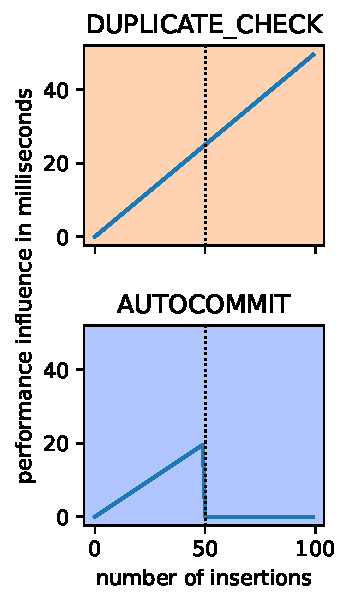
\includegraphics[width=1\linewidth]{images/influences.pdf}
	\end{subfigure}
	\caption{Illustrative example (left) with workload-dependent performance influences of configuration options \texttt{DUPLICATE\_CHECK} and \texttt{AUTOCOMMIT} (right).}
	\label{fig:intro}
\end{figure}

\subsection{Configuration-dependent Performance Modeling}
Configurable software systems are an umbrella term for any kind of software system that exhibits configuration options to customize functionality. 
While the primary purpose of configuration options is to select (categorical or binary options) and tune (numerical options) functionality, each configuration choice may also have implications on non-functional properties --- be it intentional or unintentional. Finding configurations with optimal performance~\cite{nairUsingBadLearners2017,nairFlash18,ohFindingNearoptimalConfigurations2017} and estimating the performance for arbitrary configurations of the configuration space is an established line of research~\cite{siegmundPerformanceinfluenceModelsHighly2015,haDeepPerf2019,perfAL,guoVariabilityawarePerformancePrediction2013,sarkarCostEfficientSamplingPerformance,guo_2018_data,fourier_learning_2015,perLasso}. 
Take as an example of a configurable software system the method \texttt{insertRows} in Figure~\ref{fig:intro} from an exemplary database system. It receives as an argument an array of strings, each a row to insert. 
The method exhibits two configuration options, \texttt{DUPLICATE\_CHECK} and  \texttt{AUTOCOMMIT}. If \texttt{DUPLICATE\_CHECK} is enabled, the passed array of insertion statements is checked for duplicates by  inserting all array items into a \texttt{HashSet} (\colorbox{duplicatecheck}{Lines 2--6}).
If \texttt{AUTOCOMMIT} is enabled, each insertion is treated as a single transaction (\colorbox{autocommit}{Lines 12–14}), whereas the method \texttt{commit} might otherwise be called  after  all rows have been inserted. By enabling or disabling such configuration options, the method's behavior, and, thus, its execution time changes.


Machine-learning techniques have been used to learn \emph{performance models} that approximate non-functional properties, such as execution time or memory usage, as a function of software configurations $c \in C$, formally $\Pi: C \rightarrow \mathbb{R}$.
Performance models can be obtained using a variety of machine-learning techniques, including probabilistic programming~\cite{dorn2020}, multiple linear regression~\cite{siegmundPerformanceinfluenceModelsHighly2015}, classification and regression trees~\cite{sarkarCostEfficientSamplingPerformance,guo_2018_data}, Fourier learning~\cite{fourier_learning_2015,perLasso}, and deep neural networks~\cite{haDeepPerf2019,perfAL}.
The set of configurations for training can be sampled from the configuration space using a variety of different sampling techniques. All sampling strategies aim at yielding a representative sample, either by covering the main effects of configuration options and interactions among them~\cite{siegmundPredictingPerformanceAutomated2012}, or sampling uniformly from the configuration space~\cite{ohFindingNearoptimalConfigurations2017,kaltenecker_distance-based_2019}.

Most approaches share the perspective of treating a configurable software system as a black-box model at application-level granularity. Recent work has incorporated feature location techniques to guide sampling effort towards relevant configuration options~\cite{velez_2020_configcrusher_jase,velez_comprex_2021} or model non-functional properties at finer granularity~\cite{weber_white_2021}.

\subsection{Workload-dependent Performance Modeling}

In performance and load testing, it is a common practice to select a workload that is reflective of the software system in question~\cite{ceesay2020,papadopoulos2021}. This can be achieved by constructing workloads, among others, from usage patterns~\cite{calzarossa2016}, or by increasing the workload coverage by using a mix of different workloads rather than a single one~\cite{jiang2015survey}.
The benefit of using more than one specific workload for performance models is illustrated by the work of \citeauthor{liao_2020_using_emse}~\cite{liao_2020_using_emse}. For two different versions of a software system, they learn performance models based on disjoint sets of workloads. From the comparison of both performance models, they were able to identify performance shifts as the workload bias was averaged out.

Workload-specific differences in the performance behavior of configurable software systems have been documented before~\cite{jamishidi_transfer_2017,alves_sampling_2020}. \citeauthor{jamishidi_transfer_2017} observe that performance influences across different environments remain largely congruent and differences only affect small numbers of configuration options, such that differences can be learned efficiently via transfer learning~\cite{jamishidi_transfer_2017,jamshidi_learning_2018,jamshidi_transfer_gp_2017,ding_bayesian_2020}. Here, the bias is explicitly learned to adapt an already existing --- and potentially also biased --- performance model. \citeauthor{alves_sampling_2020} have observed dissimilar performance distributions for the video transcoder \textsc{x264} over different  workloads.

To illustrate the influence that workloads can have on
configuration performance, let us revisit the introductory example from Figure~\ref{fig:intro}. In addition to being dependent on the configuration, the execution of \texttt{insertRows} also depends on its workload,  the array of insertion statements. If the array size exceeds 50 (line~50), by design all insertions are handled by another method, \texttt{insertBulkRows}. Consequently, the code section depending on option \texttt{AUTOCOMMIT} also depends on the workload size as it is skipped for arrays with more than 50 items. 
To model the performance of any execution of method \texttt{insertRows}, we have to consider the influence of the configuration options, the workload, and the interactions between both. If we assume that each insertion takes a constant amount of time, we expect the method execution time to be proportional to the number of insertion statements. For the individual configuration options, however, the workload size can distort this conception. We illustrate this facet in Figure~\ref{fig:intro}~(right), where the performance influence of both configuration options is shown as a function of the number of insertions. Here, the influence of option \texttt{AUTOCOMMIT} becomes negligible for workloads with more than 50 insertion statements. That is, any configuration  with this option enabled will behave differently depending on the workload. At large, a performance model for this database system learned with a workload of either less or more than 50 insertions cannot generalize to the respective other scenarios.


\subsection{Mapping Features to Code}\label{sec:feature_location}
The problem of determining which code implements which functionality in a software system is known as \emph{feature location}~\cite{rubin_feature_2013}. To reason about the degree to which a software feature (e.g., code conditioned by a configuration option) is covered under a workload, a mapping from features to code is necessary. 
%and can be obtained from data and control-flow analysis as well as dynamic analyses.

Most feature location approaches either employ static or dynamic program analysis to infer a mapping between features and code. As for static analyses, variables that encode configuration options (e.g., \texttt{AUTOCOMMIT} in Listing~\ref{fig:intro}) are tainted and, from tracing dataflow and controlflow, one can infer code sections tainted by such variables~\cite{velez_2020_configcrusher_jase,lillack_2018_lotrack_tse,luo_2019_cova}.
While static analyses can yield precise results, scalability is often limited by the exploration of all possible execution paths. To mitigate this shortcoming, dynamic taint analysis taints variables similarly to the static approaches, but only follows one execution path~\cite{bell_phosphor_2014,velez_comprex_2021,splat_kim_2013}. From few executions of different configurations, one can extract feature-specific code. In the context of the example in Listing~\ref{fig:intro}, two runs with \texttt{DUPLICATE\_CHECK} either enabled or disabled, respectively, would allow us to determine the lines of code depending on this option.


Aside from program analysis, a more tame, but also less precise approach is to use code coverage information, such as execution traces.
The rationale is that by exercising feature code, for instance via enabling configuration options or running corresponding tests, its location can be inferred from code coverage differences. Applications of such an approach have been studied not only for feature location~\cite{wong_integrated_2005,sulir_annotation_2015,michelon_spectrum_2021,perez_framing_2016}, but root in program comprehension~\cite{wilde_early_1996,wilde_reconnaissance_1995,sherwood_reducing_nodate,perez_diagnosis_2014,castro_pangolin_2019} and fault localization~\cite{agrawal_fault_1995,wong_faultloc_2016}. In the context of our example from Figure~\ref{fig:intro}, the feature code for options \texttt{DUPLICATE\_CHECK} (\colorbox{duplicatecheck}{Lines 2--6}) and \texttt{AUTOCOMMIT} (\colorbox{autocommit}{Lines 12–14}) could be inferred from the diff between execution traces where each option is once enabled and once disabled, respectively.


\section{Empirical Study}~\label{sec:study}
We have conducted an empirical study of a multitude of configurations and workloads for six configurable software systems. In the following, we describe the general experiment setup and study design as well as research questions and results. We make all performance measurement data, configurations, workloads, and learned performance models available on this paper's companion Web site.\todo{Coverage data raw or available at other third party platform than github?}

\subsection{Experiment Setup}\label{sec:setup}
\paragraph*{Subject Systems and Workloads}
For our study, we have selected six configurable software systems implemented in Java. We decided to use Java for mainly two reasons: (1) practically, because we can forgo code modifications for instrumentation by using off-line instrumentation (cf.~Section~\ref{sec:profiling}) for code coverage measurement, and (2) strategically, because Java is one of the most widely used programming languages. We discuss this decision in more detail in Section~\ref{sec:threats}. 
The full list of our subject systems and characteristics is presented in Table~\ref{tab:subject_systems}. Due to space limitations, we provide a more extensive description of the used workloads at the paper's companion Web site. While we have measured more than one performance metric for all configurable software systems (except for \htwo), in the following we focus on response time and throughput to keep our analysis comparable. All measurements are available at the paper's companion Web site.
	
\jumper is a re-implementation of the LAME audio codec for MP3 in Java. In total, we have selected six WAVE audio files as a workload to encode to MP3. To diversify the selection of workloads, we indcluded audio files with different characteristics (sampling rate, number of channels, length, etc.). 
\kanzi is a file compression tool. For this subject system, we selected nine workloads, including, among others, dedicated compression benchmarks (sets of files of different types) as well as binary and text files at different scales: a binary of the Linux kernel, a dump of its repository, XML and CSV data. 
\dconvert is a Java utility to scale images for use in Android apps into different formats and different resolutions. For our experiments, we selected a range of workloads, varying in file type (JPEG, PNG, PSD, and SVG) and size.
\batik is a Java utility to rasterize vector graphics, for which we selected a range of workloads varying in size.
\jadx is a decompiler and deobfuscator for Android applications, for which we selected a range of popular APK packages as workloads, varying in application domain and size.
\htwo is a relational database that can be integrated into Java applications or used as a standalone database. We used a selection of application-level benchmarks from the \textsc{OLTPBench}~\cite{difallah_oltp_2013}, a load generator for databases that allows for testing benchmarks, such as \textsc{TPC-C}. Overall, the selection of the workloads was driven by diversity to make use of different functionality of a subject system and by size to probe for scaling and utilization factors.
	
\begin{table*}[ht!]
		\centering
		\caption{Subject system characteristics}
		\begin{tabularx}{\linewidth}{lllrrrr}
		\toprule
		\textbf{Software System} &  \textbf{Application Type} & \textbf{Revision} & \textbf{ \#\,O} & \textbf{\#\,C} & \textbf{\#\,W}  \\
		\midrule
		\jumper & Audio encoder & 1.0.4 & 19 & 4\,196 & 6   \\
		
		\kanzi & File compressor & 1.9 & 24 & 4\,112 & 9 \\
			
		\dconvert & Image scaling & 1.0.0-alpha7 & 17 & 6\,764 & 12  \\
				
		\htwo & Embedded database & 1.4.200 & 16 & 1\,954  & 8  \\
		
		\batik & SVG rasterizer & 1.14 & 10 & 1\,919 &  11  \\
		
		\jadx & Java decompiler & 1.2.0 & 18 & 10\,502 & 9  \\
\bottomrule

\end{tabularx}\\
{\vspace{1mm}\textit{Abbreviations: \#\,O: No. of options, \#\,C: No. of configurations, \#\,W: No of. workloads}}

		\label{tab:subject_systems}
	\end{table*}

\paragraph*{Configuration Sampling}\label{sec:sampling}
For each subject system, we sampled a set of configurations. Exhaustive coverage of the configuration space is infeasible due to combinatorial explosion~\cite{henardCombining2015}. We combine several coverage-based sampling strategies and uniform random sampling into an \emph{ensemble} approach: To study the influence of single configuration options, we employ option-wise and negative option-wise sampling~\cite{siegmundPerformanceinfluenceModelsHighly2015}, where each option is enabled once, or all except one, respectively. In the same way, pair-wise sampling applies this schema to study influences of two-way interactions between configuration options. Interactions of higher degree can be found accordingly, which, however, is computationally prohibitively expensive~\cite{henardCombining2015}. Instead, we augment our sample set with a random sample that is, at least, twice the size of the coverage-based sample. To achieve a uniform random sample, we used \emph{distance-based sampling}~\cite{kaltenecker_distance-based_2019}. The variability models, as well as sample sets, can be found on the paper's companion Web site.
	
\paragraph*{Coverage Profiling}\label{sec:profiling}
To measure code coverage, we use the on-the-fly profiler \textsc{JaCoCo}. Unlike profilers that use source code instrumentation, with on-the-fly instrumentation, the executable binary remains unchanged. This way, we avoid altering and re-compiling the source code or injecting instrumentation code post compilation. From a practical perspective, on-the-fly instrumentation is more flexible and easier to accommodate. Nonetheless, either choice introduces some performance overhead. To avoid this overhead distorting our performance measurements, we conducted our coverage analysis in a separate run, for which no performance data was collected. 	
	
\paragraph*{Hardware Setup}
All experiments were conducted on three different compute clusters and each subject system was exclusively run on a single cluster. All machines in a compute cluster had the identical hardware setup: either with Intel~Core~i5-8259U CPUs at 2.3~GHz (\jumper and \kanzi),  Intel~Core~i7-8559U CPUs at 2.7~GHz (\dconvert, \batik, and \jadx) and 32~GB of RAM, respectively, or Intel~Xeon~E5-2630~v4 CPUs at 2.2~GHz with 256~GB of RAM (\htwo). All clusters ran a headless Debian 10 installation, the first two with kernel version \mbox{\texttt{4.19.0-14}}, the latter with version \mbox{\texttt{4.19.0-17}}. 
To minimize measurement noise, no additional user processes were running in the background, and no other than necessary packages were installed.	For all data points, we report the median across five repetitions (except for \htwo), which has shown to be a good trade-off between variance and measurement effort. {\color{red}For \htwo, we omitted the repetitions as in a pre-study, running on the identical cluster setup, we found that across all benchmarks the throughput coefficient of variation (standard deviation divided by the arithmetic mean) was consistently below~5\,\%.\todo{why sufficient? could be weak point, maybe reference other work employing a similar threshold} }


\subsection{Workload-specific Configuration Performance}\label{sec:rq1}
It is well known that performance variation can arise from differences in the workload~\cite{benchmarking_book}. 
This has been observed as well for software systems in the presence of configuration options, such as for the video encoder x264~\cite{alves_sampling_2020}. \citeauthor{alves_sampling_2020} show that, under two different workloads, the configuration-specific performance behavior of x264 varies widely. 

%{\todo{fuzzy}\color{orange}For example, while the set of performance observations over a selection of configurations of \textsc{x264} observed by  exhibit little to no similarity to each other, for another series of subject systems, the influences of options (or their order) remained mostly stable, while only few shifted~\cite{jamshidi_transfer_gp_2017,jamishidi_transfer_2017}.}  The similarity between workload-specific performance distributions observed by \citeauthor{jamshidi_learning_2018} is key to adapt existing performance models to a new workload~\cite{jamshidi_learning_2018}. 

In a practical setting, the question arises whether, and if so, to what extent an existing workload-specific performance model is representative of the performance behavior of other workloads as well. 
That is, can a model estimating performance of different configurations be reused for the same software system, but learned under a different workload?
Depending on the degree of similarity, such a performance model could be either (1) re-used, (2) transformed at a reasonable cost, or (3) must be re-learned entirely, which entails a substantial measurement cost. To provide some context for the feasibility of model reuse or transformation, we formulate the following research question: 

\RQ{1}{To what extent does performance behavior vary across workloads?}

\paragraph*{Operationalization}
We address this research question by comparing workload-specific performance distributions obtained from our experiments (cf. Section~\ref{sec:study}). To this end, we investigate whether any two distributions obtained from two different workloads can be transformed into each other, or are not related in any way. As no single-valued metric can reliably describe the above properties, we employ an aggregate of multiple metrics: 

If the distributions can be transformed using linear transformation, such as scaling and shifting, we expect a high linear correlation, which we measure by Pearson’s correlation coefficient (\emph{Pearson's~r}). As an additional metric, we use Kendall’s rank correlation coefficient (\emph{Kendall's~$\tau$}) to test for further possible transformations. As rank correlation usually subsumes linear correlation, a low linear but high rank correlation indicates that only a non-linear transformation is possible. In the case where rank correlation does not indicate a relationship, we consider the distributions dissimilar. From these three metrics, we classify the pairs of workload-specific distributions into three different categories:
\vspace{1mm}

\begin{tabular}{p{4.4cm}l}
	 \textbf{Category} & \textbf{Criteria} \\
	{linearly transformable (LT)} & $r \geq 0.6$ \\
	{monotonically transformable (MT)} & $r < 0.6$, and $\tau \geq 0.6$ \\
	{dissimilar}  & (otherwise) \\%$p < 0.05$ and $\tau < 0.6$ \\
\end{tabular}

\paragraph*{Results}
We found that the performance behavior of the six configurable software systems varied widely. We illustrate the results in Table~\ref{tab:categorization}. For half of the software systems (\kanzi, \batik, and \jadx), in the majority of workload pairs, the resulting performance distributions could be transformed using a linear transformation. For \jumper, more than half of the workload pairs are accountable to monotonic transformation. For \dconvert and \htwo, the majority of workload comparisons resulted in dissimilar performance distributions, however, a substantial amount was linearly transformable. For \jumper and \jadx, we found no case of non-transformable performance distributions, whereas the other four software systems exhibited dissimlar performance distributions under, at least, one workload. For \jadx, all performance distributions were linearly transformable.

In Figure~\ref{fig:diff_performance_similarity}, we provide a more detailed breakdown of which workloads resulted in performance distributions dissimilar to other ones in terms of a correlation matrix (Kendall's $\tau$) for each pair of workloads. Notable for \dconvert is the behavior for SVG workloads (and one JPG workload), which resulted in distributions dissimilar to the remaining workloads. For \htwo, the workloads \texttt{ycsb-2400} and \texttt{tpcc-8} are dissimilar to all other workloads, including their counterparts with a lower scalefactor (600 and 2, respectively).

\begin{table}
	\caption{Category counts of configuration-specific performance for workload pairs}
	\begin{tabular}{p{2.4cm}rrr}
		\toprule
		\textbf{Software System} & \textbf{LT} & \textbf{MT} & \textbf{dissimilar}\\
		\midrule
		\jumper &  7 (46.6\,\%) & \cellcolor{nicegreen!20}8 (53.3\,\%)& 0 (0\,\%)\\
		\kanzi &  \cellcolor{nicegreen!20}28 (77.8\,\%)& 4 (11.1\,\%) & 4 (11.1\,\%)\\
		\dconvert &  29 (43.9\,\%) & 0 (0\,\%) & \cellcolor{nicegreen!20}37 (56.0\,\%)\\
		\htwo &  11 (39.3\,\%) & 0 (0\,\%) & \cellcolor{nicegreen!20}17 (60.7\,\%)\\
		\batik &  \cellcolor{nicegreen!20}28 (50.9\,\%) & 8 (14.5\,\%) & 19 (34.5\,\%)\\
		\jadx  &  \cellcolor{nicegreen!20}120 (100\,\%) & 0 (0\,\%) & 0 (0\,\%)\\
		\bottomrule
	\end{tabular}
	\label{tab:categorization}
	
	{\vspace{2mm}
		{\footnotesize Abbreviations:$\quad$LT: \textit{Linearly transformable}, MT: \textit{Monotonically transformable}}
	\vspace{0.1cm}}
	
\end{table}

\begin{figure*}
	\centering
	\begin{subfigure}{0.33\textwidth}
		\centering
		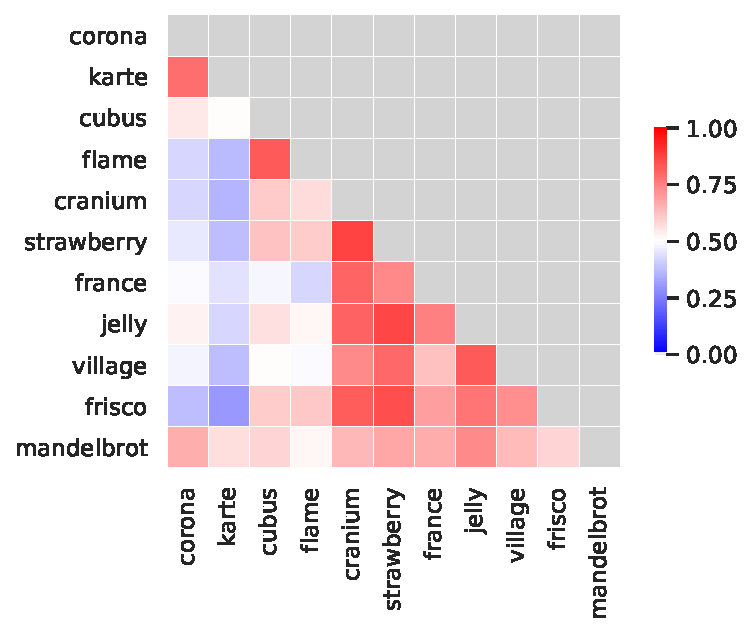
\includegraphics[width=\linewidth]{images/rq1/kendall_batik.pdf}
		\caption{\batik}
	\end{subfigure}
	\begin{subfigure}{0.33\textwidth}
		\centering
		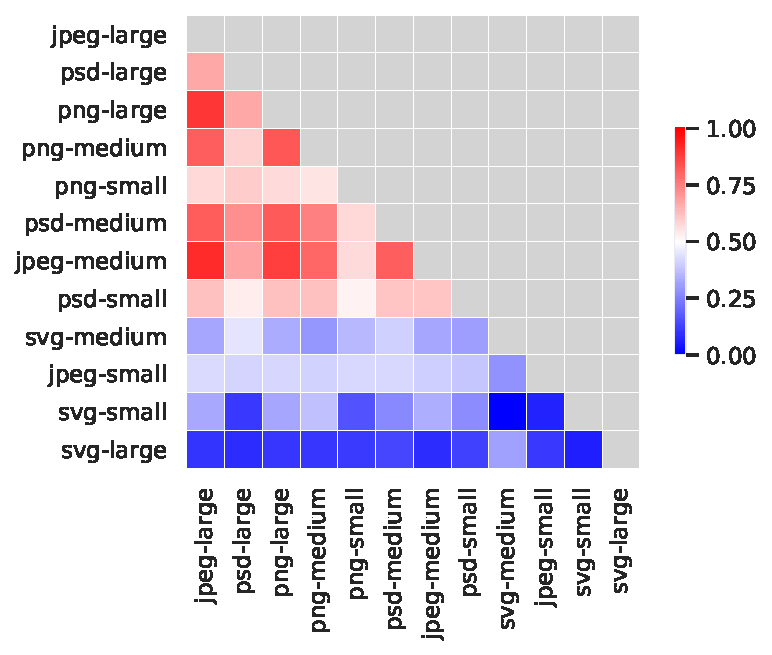
\includegraphics[width=\linewidth]{images/rq1/kendall_dconvert.pdf}
		\caption{\dconvert}
	\end{subfigure}
	\begin{subfigure}{0.33\textwidth}
		\centering
		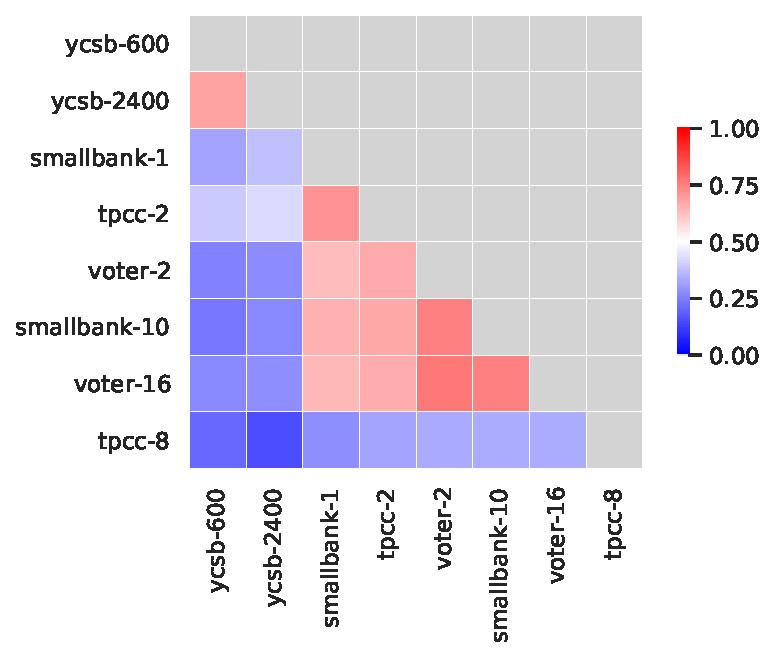
\includegraphics[width=\linewidth]{images/rq1/kendall_h2.pdf}
		\caption{\htwo}
	\end{subfigure}
	\begin{subfigure}{0.33\textwidth}
		\centering
		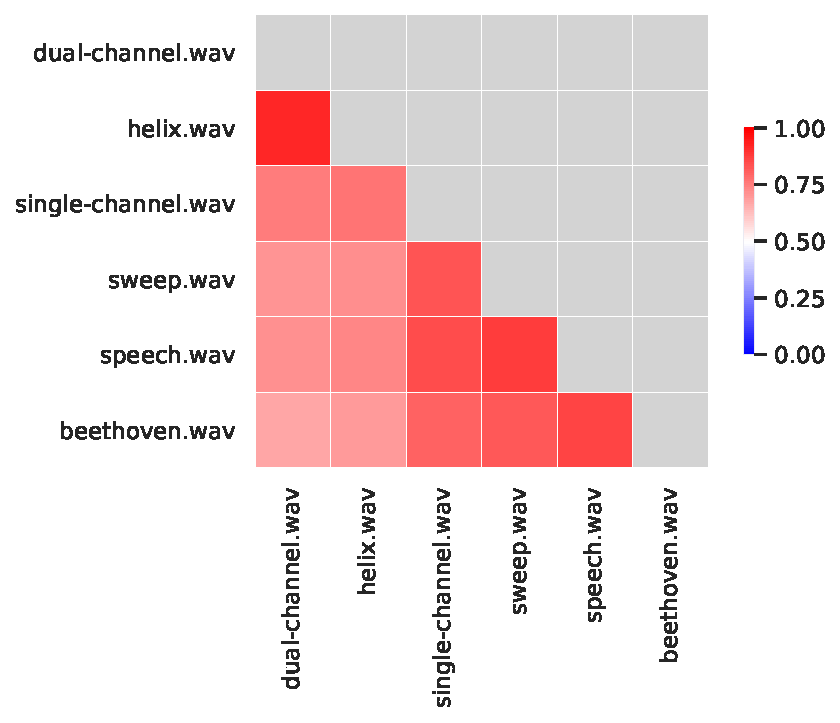
\includegraphics[width=\linewidth]{images/rq1/kendall_jump3r.pdf}
		\caption{\jumper}
	\end{subfigure}
	\begin{subfigure}{0.33\textwidth}
		\centering
		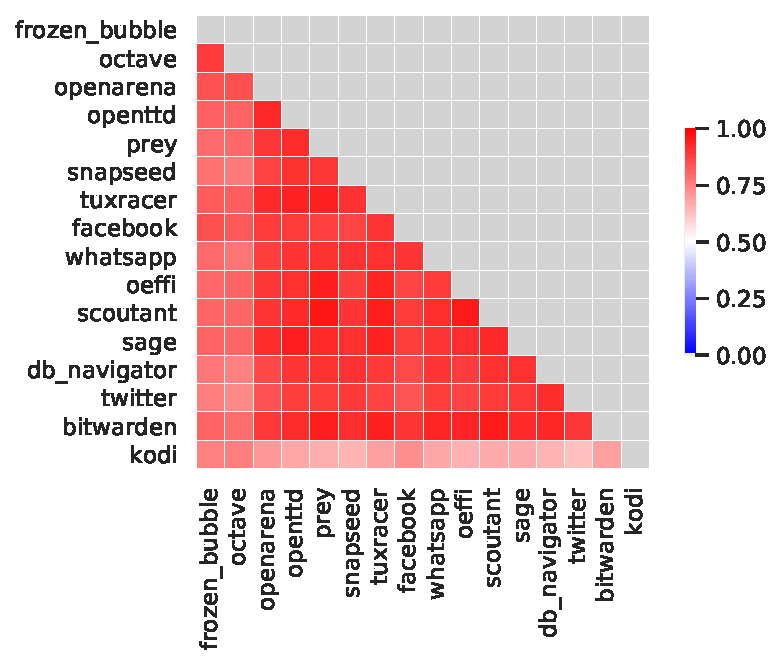
\includegraphics[width=\linewidth]{images/rq1/kendall_jadx.pdf}
		\caption{\jadx}
	\end{subfigure}
	\begin{subfigure}{0.33\textwidth}
		\centering
		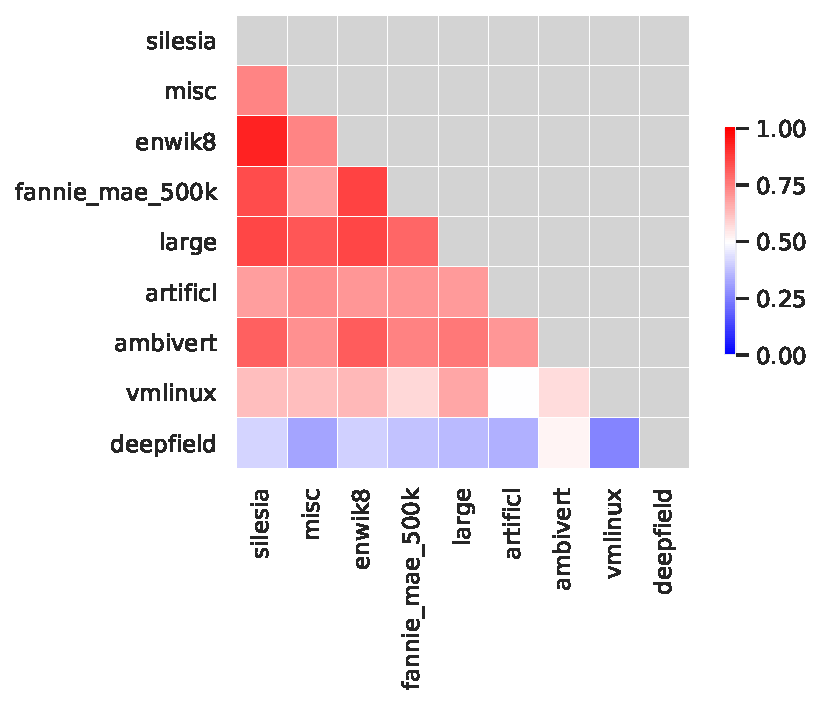
\includegraphics[width=\linewidth]{images/rq1/kendall_kanzi.pdf}
		\caption{\kanzi}
	\end{subfigure}
	\caption{Similarity matrix (Kendall's $\tau$) for performance distributions of different pairs of workloads.}
	\label{fig:diff_performance_similarity}
\end{figure*}
\vspace{1em}
\greybox{\textbf{Summary} (\RQref{1}): Not all software systems' performance behavior changes similarly across workloads. For \dconvert, performance behavior under SVG workloads is different to most other workloads, and for \htwo, performance behavior under workloads with higher scale factors is more likely to be dissimilar to behavior under other workloads.}\todo{Discussion with Florian}


\subsection{Performance Model Similarity}\label{sec:rq2}
Our categorization of the differences between workload-specific performance distributions does help understand the degree of workload-dependent performance variation, but leaves out the role of configuration options. From a practical perspective, it is important to ask whether all configurations of a software system are equally likely to be affected by a workload choice or whether the selection of some configuration option increases or decreases this likelihood. If some configuration options show to be more sensitive to workload choices, practitioners can incorporate this knowledge into selecting configurations for regression testing or to adapt existing performance models~\cite{jamshidi_learning_2018}. To provide a clearer picture of the influence of workload variability in the presence of configuration options, we ask the following research question:

\RQ{2}{To what extent do influences of individual configuration options depend on the workload?}

\paragraph*{Operationalization}
We address this research question by learning and comparing performance models from the measurements of our experiments~\cite{dorn2020,siegmundPerformanceinfluenceModelsHighly2015,haDeepPerf2019,perfAL,guoVariabilityawarePerformancePrediction2013,sarkarCostEfficientSamplingPerformance,guo_2018_data,fourier_learning_2015,perLasso}. As a performance model effectively estimates the influence of individual configuration options on performance, we construct models not to predict unseen configurations but simply to explain differences observed in the performance distributions. So, for the construction of our performance models, we deliberately learn performance models using the entire sample set. 
To correct for multicollinearity~\cite{Daoud_2017} and to ensure that the obtained performance influences are interpretable, we drop several configuration options from the sample set, which has shown to be an effective practice~\cite{dorn2020}. For the training step, we exclude all mandatory configuration options since these by definition cannot contribute to performance variation. In addition, for each group of mutually exclusive configuration options, we discard one randomly selected group member.

Many different machine learning techniques have been used to obtain performance models, among others, based on linear regression~\cite{perLasso,siegmundPerformanceinfluenceModelsHighly2015,dorn2020}. To answer \RQref{2}, we learn a prediction model using multiple linear regression (least-squares method). We limit the set of independent variables to individual options rather than higher-order interactions to be consistent with the feature location used for \RQref{3.2} where we determine option-specific, but not interaction-specific code segments

From the comparison of the performance model coefficients, we can answer \RQref{2} in detail and assess (1) how many configuration options, on average, change their influence, and (2) how many configuration options, in total, change their influence. For any pair of workload-specific performance models, we divide the performance model coefficients by the respective mean performance to make the model influences comparable across workloads. Henceforth, we will refer to these coefficients as \textit{relative performance influences.} Since these relative performance influences have been divided by the population mean, we report these without any unit.

\begin{table}
	\centering
	\caption{Absolute number of configuration options whose relative performance influence changed by at least by threshold $t$ under, at least, one workload configuration.}
	\begin{tabular}{lr|rrrrr}
		\toprule
		& &  \multicolumn{5}{c}{\textbf{Difference threshold $t$}} \\
		\textbf{Software System} & \textbf{\#\,Opt.} & 0.01 &  0.05 &  0.1 &  0.2 &  0.5 \\
		\midrule
		\dconvert & 23 &    14 &    12 &    7 &    6 &    1 \\
		\jumper & 36 &   30 &    29 &   29 &   25 &    9 \\
		\batik &  20 &  10 &     7 &    6 &    6 &    5 \\
		\kanzi & 29 &   26 &    26 &   25 &   20 &    9 \\
		\jadx & 20 &   19 &     9 &    5 &    4 &    2 \\
		\htwo & 17 &   16 &     5 &    3 &    1 &    0 \\
		\bottomrule
	\end{tabular}
	\label{tab:total_changes}
\end{table}
\begin{table}
	\caption{Average number of configuration options whose relative performance influence changed by, at least, by threshold $t$ across all workload combinations.}
	\begin{tabular}{lr|rrrrr}
		\toprule
		& & \multicolumn{5}{c}{\textbf{Difference threshold $t$}} \\
		\textbf{Software System} & \textbf{\#\,Opt.} & 0.01 &  0.05 &  0.1 &  0.2 &  0.5 \\
		\midrule
		\dconvert & 23 &  8.89 &  5.29 &  3.55 &  1.65 & 0.09 \\
		\jumper & 36 & 24.73 & 19.87 & 16.27 & 11.40 & 4.33 \\
		\batik & 20 &  7.22 &  4.47 &  3.62 &  2.95 & 1.18 \\
		\kanzi & 29 & 23.61 & 15.83 & 10.33 &  6.33 & 2.56 \\
		\jadx & 20 & 10.32 &  4.28 &  2.51 &  1.38 & 0.33 \\
		\htwo & 17 & 7.39 &  2.43 &  1.04 &  0.43 & 0.00 \\
		\bottomrule
	\end{tabular}
	\label{tab:average_changes}
\end{table}

\paragraph*{Results} 
We show the distribution of the relative performance model coefficients in the box plots in Figure~\ref{fig:feature_influence_actross_workloads}. We see that, for all software systems, only a small number of configuration options influences performance. While for most configuration options, we observe substantial workload-specific variation if they are influential options. Notably though, for \dconvert (option \texttt{png}) and \kanzi (e.g., option \texttt{BWT}), we see that otherwise non-influential options become influential. Moreover, for \batik, \dconvert, and \kanzi, we observe a large number of outliers, which indicates that for these software systems, some options' performance influence can be quite workload-specific.
To further quantify the cases of such volatile configuration options, we break down the numbers of how many configuration options changed in Tables~\ref{tab:total_changes} and~\ref{tab:average_changes}. In Table~\ref{tab:average_changes}, we present the total number of configuration options whose relative performance influence was different in, at least, one comparison of workload-specific performance models. IN place of a fixed absolute difference threshold, we report the number of configurations at five different thresholds. For \jumper and \kanzi, more than half of the configuration options' influences changed, at least, by $0.2$, whereas, for the remaining software systems, less than half of the options were affected.

In this vein, we show the \textit{average} number of configuration options whose influence changed, at least, by $t$ in Table~\ref{tab:average_changes}. We see that, across all software systems and thresholds, the average number of configuration options is consistently and substantially lower than the total number of configuration options from Table~\ref{tab:total_changes}. This indicates that not for all workload pair comparisons the same number of configuration options has changed their influence. Notable is that, for the systems for which we observed a large share of dissimilar performance distributions in \RQref{1}, \dconvert, and \htwo, only a few configuration options appear to be influenced by the choice of workloads.

\begin{figure*}
	\begin{minipage}{0.33\textwidth}
		%\centering
		\begin{subfigure}{\linewidth}
			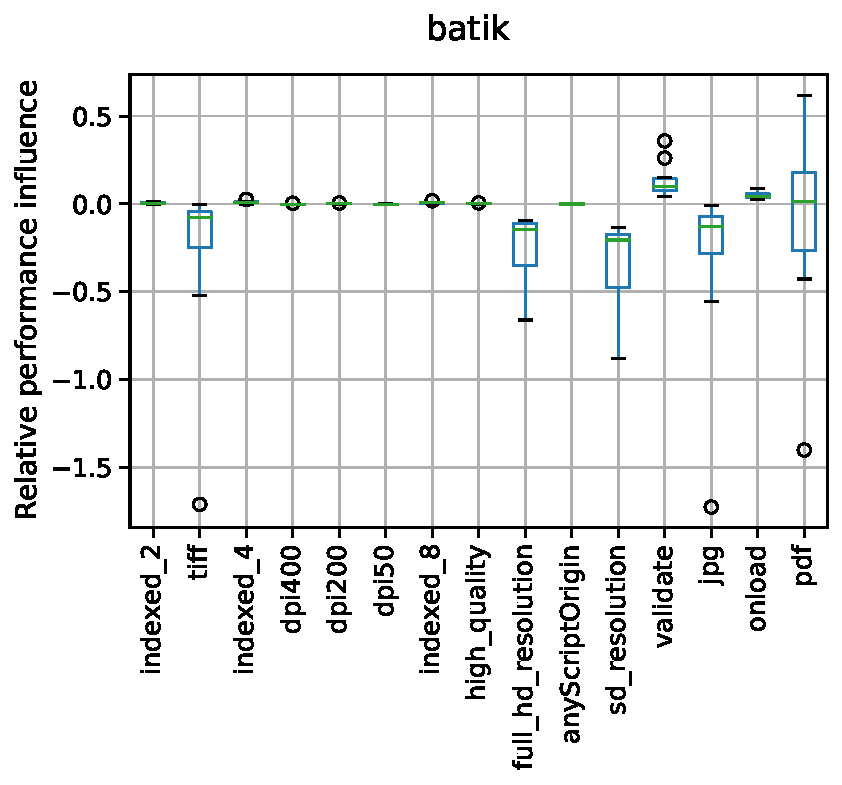
\includegraphics[width=\linewidth]{images/rq2/relative_performance_batik.pdf}			
			\vspace{15mm}
		\end{subfigure}
	\end{minipage}
	\begin{minipage}{0.33\textwidth}
		\begin{subfigure}{\linewidth}
			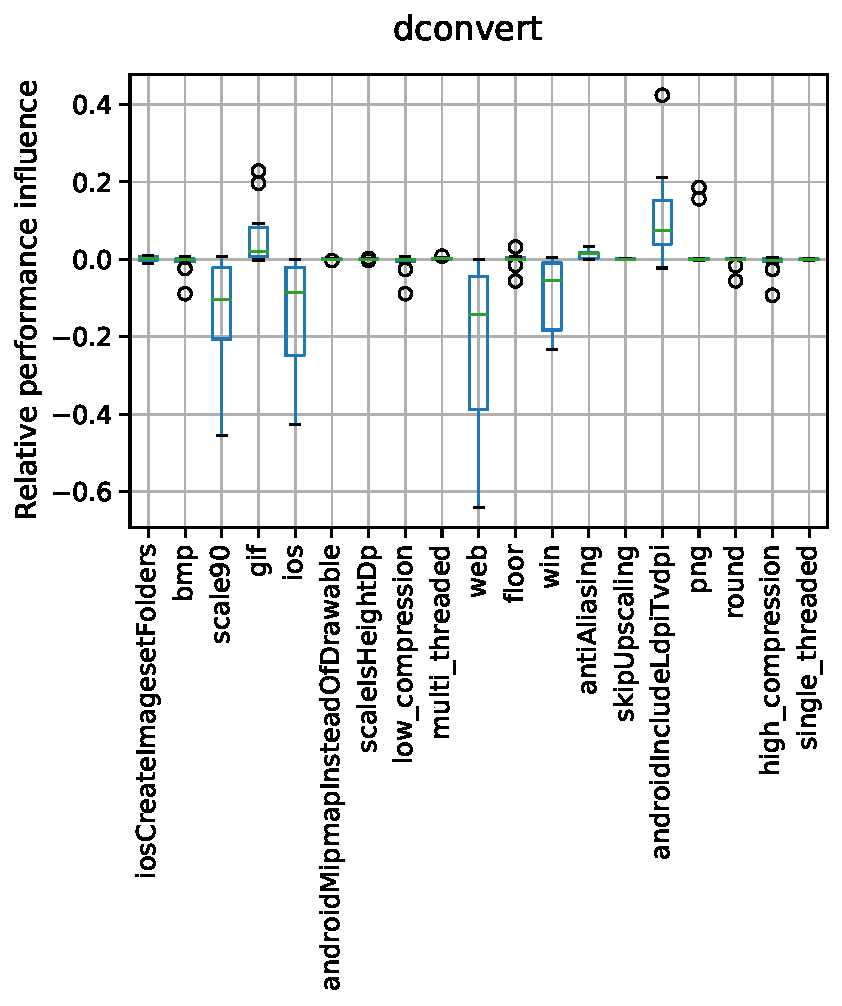
\includegraphics[width=\linewidth]{images/rq2/relative_performance_dconvert.pdf}
			\vspace{0.0001mm}
		\end{subfigure}
	\end{minipage}
	\begin{minipage}{0.33\textwidth}
		\begin{subfigure}{\linewidth}
			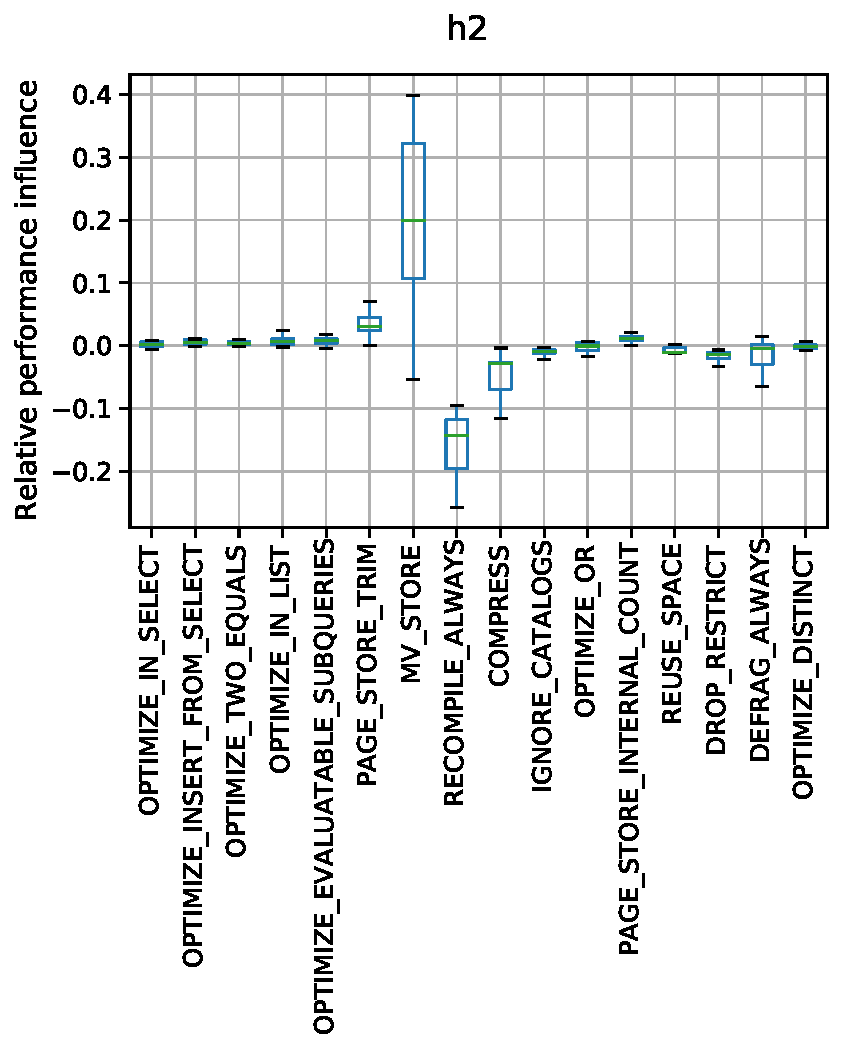
\includegraphics[width=\linewidth]{images/rq2/relative_performance_h2.pdf}

		\end{subfigure}
	\end{minipage}

	\begin{minipage}{0.33\textwidth}
		\begin{subfigure}{\linewidth}
			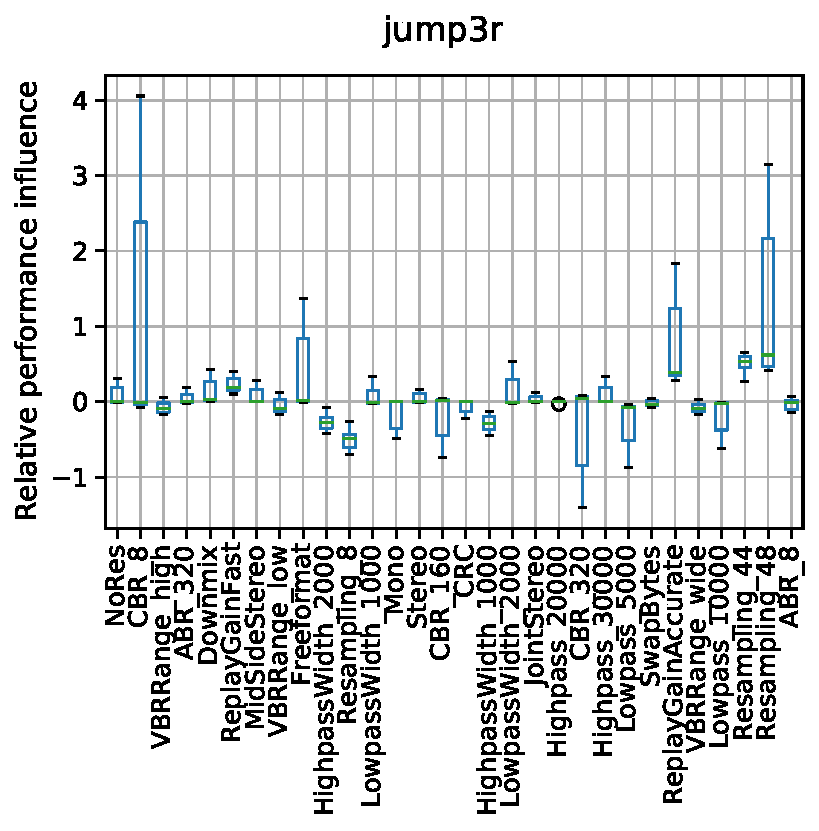
\includegraphics[width=\linewidth]{images/rq2/relative_performance_jump3r.pdf}
			\vspace{6mm}
		\end{subfigure}
	\end{minipage}
	\begin{minipage}{0.33\textwidth}
		\begin{subfigure}{\linewidth}
			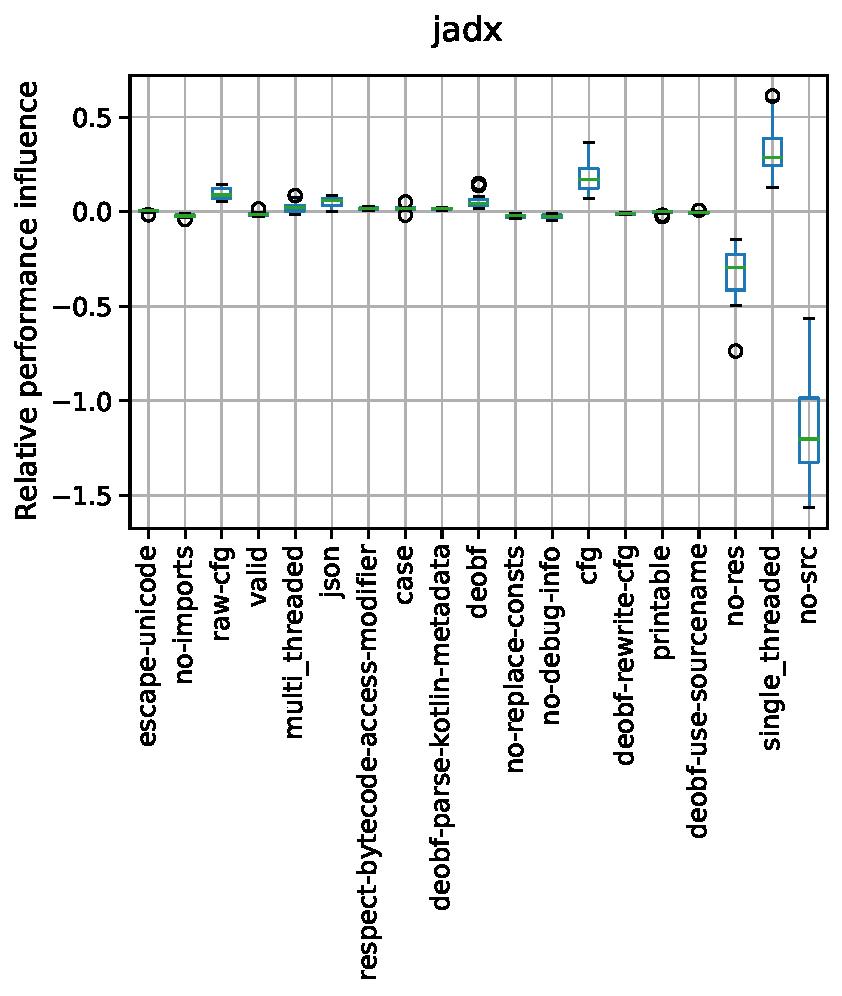
\includegraphics[width=\linewidth]{images/rq2/relative_performance_jadx.pdf}
		\end{subfigure}
	\end{minipage}
	\begin{minipage}{0.33\textwidth}
		\begin{subfigure}{\linewidth}
			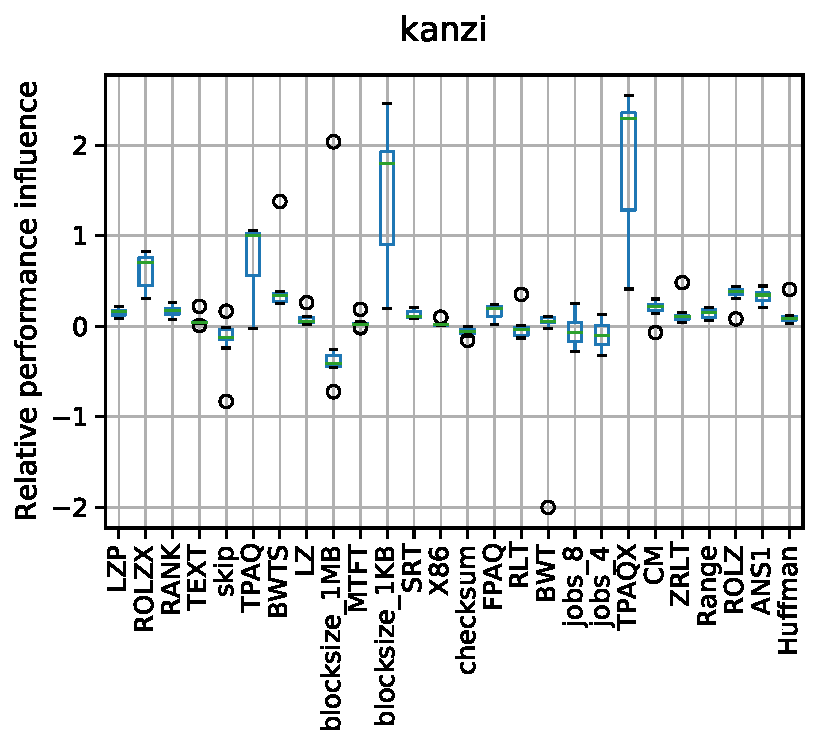
\includegraphics[width=\linewidth]{images/rq2/relative_performance_kanzi.pdf}
			\vspace{1.19cm}
		\end{subfigure}
	\end{minipage}
	\caption{Relative performance influence distribution across workloads per software system.}
	\label{fig:feature_influence_actross_workloads}
\end{figure*}

\vspace{1em}
\greybox{\textbf{Summary} (\RQref{2}) Most workload-specific variation affects influential configuration options, while some workloads let some options become influential. For most software systems, less than 50\,\% of configuration options' influence changed substantially depending on the workload. For systems with a high variation in performance behavior across workloads (cf.~\RQref{1}), only a few configuration options' influence depends on the workload.}


\subsection{Code Coverage and Performance}\label{sec:rq3}
{\color{red!50!black}
Our analysis of the effects of workload variation so far has taken only black-box measurements into account. In addition, we want to know whether the sensitivity of different configuration options (or interactions) to workload variation manifests itself only in performance differences, or if it can be understood at a finer granularity and travel back to the level of code. To draw parallels with software testing, where we determine which code is actually executed, we now extend our perspective on the problem with statement coverage data. 

%The rationale behind this is that performance emerges, among others\footnote{The hardware setup is plausibly a deciding factor for performance behavior as well~\cite{jamishidi_transfer_2017}, but was not varied in this experiment. We discuss this limitation in the threats to validity.}, from configuration and workload choice.

For illustration, let us revisit the introductory example from Figure~\ref{fig:intro}, where \colorbox{duplicatecheck}{Lines 2--6} depend on the selection of configuration option \texttt{DUPLICATE\_CHECK}. Once selected, its influence is proportional to the number of queries to handle. By contrast, the invocation of the method \texttt{insertBulkRows} later on solely depends on the number of queries exceeding the minimum of 50 queries. While both examples exhibit workload-specific behavior, the execution in the former depends on the configuration option and the latter example depends on workload properties. 
For practitioners, understanding not only whether but also, how configuration options interact with the workload is useful for assessing a performance model with regard to representativeness. 

To start to translate our findings of performance variation under varying workloads into actionable strategies, we require insights about where and how workloads and configurations interact. For instance, if a performance model is based on code segments that are covered only under a specific workload, it incorporates some workload bias. Consequently, the model cannot make accurate predictions for performance behavior under another workload, where different code segments can be executed. Likewise, if performance-relevant code is covered under a variety of workloads, but each workload stressed this code segment differently, the performance influence is likely biased by each individual workload, rendering each workload's performance model unrepresentative. Knowing where (for which options) and how (by option-code coverage or option code usage) configurations and workloads interact, paves an avenue towards actively searching for workloads that increase utilization or maximize coverage.

In the last part of this evaluation, we shed light on this aspect and explore the relationship between the execution of configurable software systems and the observed performance and answer the following research question:


%\RQ{3}{To what extent do varying workloads influence both performance behavior and set of covered code lines?}
\RQ{3}{To what extent do individual options' influence on performance and option-specific code coverage depend on the workload?}\todo{schwer zu verstehen}

\paragraph*{Operationalization (RQ~3)}
To approach the research question, we compare each option's performance influence and option-specific code coverage across pairs of workloads. 
To determine which code can be attributed to individual configuration options, we employ a two-step process. First, we obtain a baseline of all code that depends on a configuration option within the scope of our entire benchmark selection. For each workload $w \in W$, we compute the set of code lines that depend on option $o \in O$. Let $C_{o}$ be the set of configurations with option $o$ selected, and $C_{\neg o}$ with option $o$ deselected. To obtain $S_{w, o}$, we follow a strategy similar to \textit{spectrum-based feature location}~\cite{michelon_spectrum_2021} (cf. Section~\ref{sec:feature_location}) and subtract the set of the code lines covered under $C_{\neg o}$ from those of $C_{o}$:

\begin{equation}%\todo{example from Figure~\ref{fig:intro}}
	S_{w, o} = \bigcup_{p \in C_{o}} S_{w}(p) ~ \setminus ~ \bigcup_{q \in C_{\neg o}} S_{w}(q)
\end{equation}

While $S_{w, o}$ yields an approximation of option-dependent code for a single workload, we aggregate the approximations for each workload $w \in W$ to obtain the set of lines that depend on a configuration option $o$ and are executed in, at least, one workload,~$S_{o}$. 

\begin{equation}
	S_{o} = \bigcup_{w \in W} S_{w, o}
\end{equation}

While this aggregated set is not a ground truth, it enables us to reason about differences in option-dependent code within the scope of our selected workloads. That is, the expressiveness of this baseline depends on the diversity of the workloads in question. We discuss this limitation in Section~\ref{sec:threats}. From the ratio of option-dependent code per workload to option-dependent code across workloads, $\mid S_{w_1, o}\mid/~{\mid S_{w_2, o}\mid}$, we can estimate the coverage of option-dependent code. By comparing the sets $S_{w_1, o}$ and $S_{w_2, o}$ for any two workloads $w_1$ and $w_2$, we can estimate similarity between the option-code coverage.

}
\paragraph*{Results}
{\color{red!50!black}
In Figure~\ref{fig:diff_performance_option_coverage}, we show, for all combinations of two workloads, the relationship between the similarity in option-specific code coverage on the x-axis and the difference between the option's relative performance influence (from the performance models obtained for \RQref{2}). Alongside the scatter plots for each software system, we provide histograms of the marginal distributions of both dimensions. 
Notably, for \batik, \dconvert and \jumper, we observe both high and low similarity among workload-specific coverage of option-code. For \htwo and \jadx, most workloads appear to cover disjoint parts of the option-specific code, whereas for \kanzi, most workloads show high similarity in the coverage of option-specific code. 
Regarding performance influence variation, \dconvert and \jadx show a clear picture. For \dconvert, variation is completely independent of option-code coverage. For \jadx, most performance influence variation occurs when no similar code is executed. In the light of the results from \RQref{2}, where only a few options for \jadx are influential and exhibit notable variation, the majority of perormance influence variation is accounted for by these options. A trend similar to \jadx can be seen for \jumper, although it is less pronounced as the performance influence differences for a code coverage similarity of 1 are still substantial. 
The same trend as for \jadx, but in the opposite direction, can be seen for \htwo and \batik, where performance influence variation is highest for higher option-code coverage similarities. We cannot draw a clear picture for \kanzi, where we observe little variation in option-specific code coverage.

{The results for \dconvert and \jadx are the most extreme cases that we observe. For \jadx, we can infer that option-code of the influential options is either executed or not, depending on the workload since most substantial variation is present for workload pairs that share no option-specific code coverage. For \dconvert, on the other hand, at various levels of option-code coverage similarity of pairs of workloads, we observe performance influence variation. That is, the latter is likely dominated by \textit{how} the feature code is executed.}\\
}
\greybox{\textbf{Summary} (\RQref{3}):

	\color{red}Across the six software systems, we observe a wide variety of workload-specific effects on performance influences and option-specific code coverage. Depending on the workload, software system, and configuration option, option-code coverage (as in the case of \jadx) or option-code utilization (as in the case of \kanzi) can explain workload-specific performance variation.
}

\begin{figure*}

	\begin{subfigure}{0.33\textwidth}
		\centering
		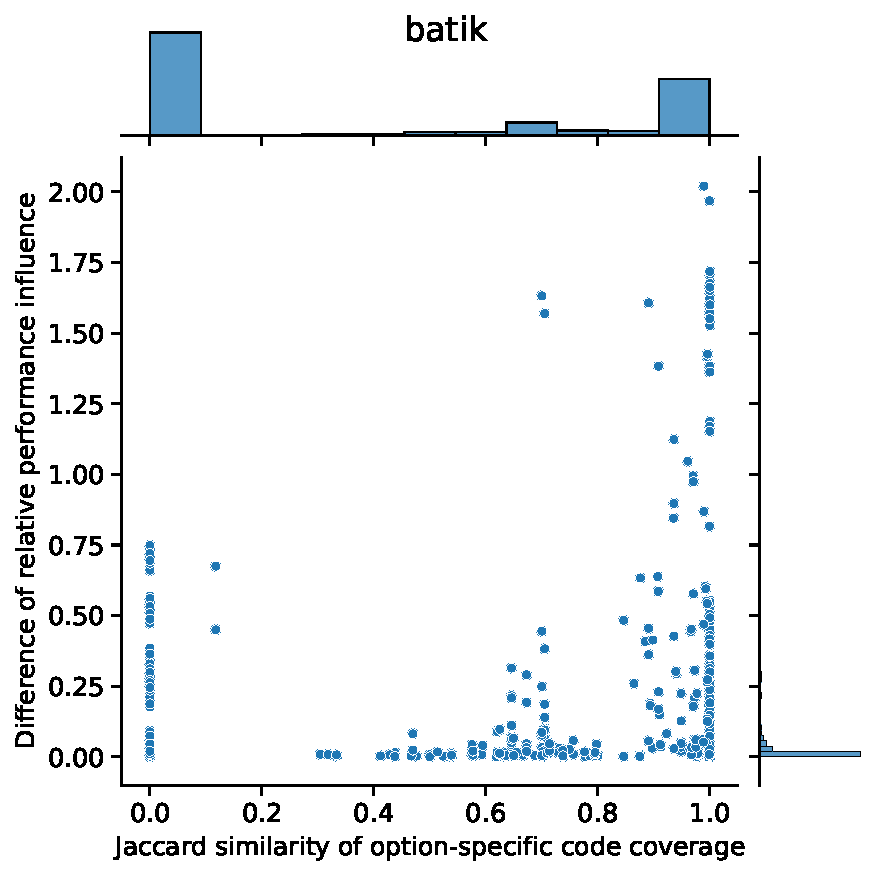
\includegraphics[width=\linewidth]{images/rq3.2/batik_rq3.2.pdf}
		%\caption{\batik}
	\end{subfigure}
	\begin{subfigure}{0.33\textwidth}
		\centering
		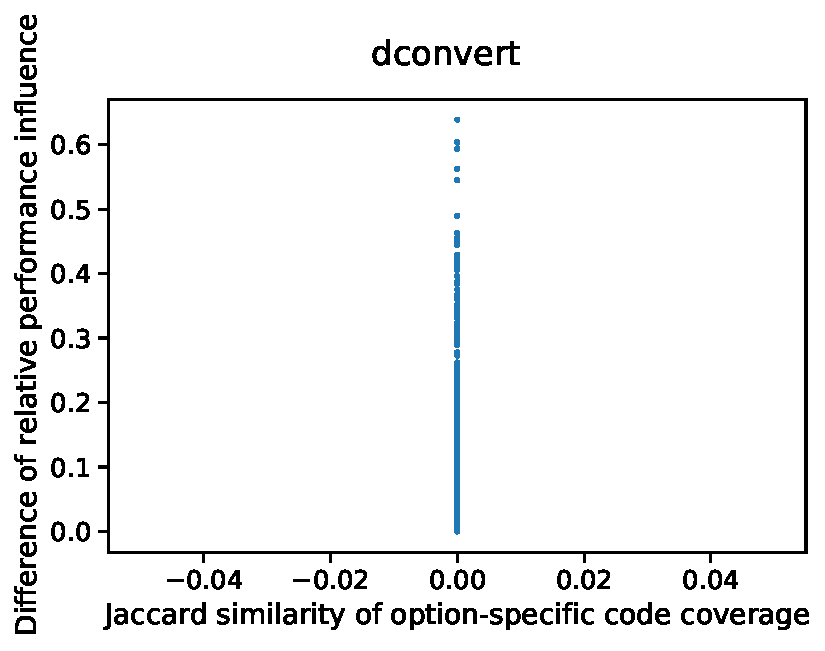
\includegraphics[width=\linewidth]{images/rq3.2/dconvert_rq3.2.pdf}
		%\caption{\dconvert}
	\end{subfigure}
	\begin{subfigure}{0.33\textwidth}
		\centering
		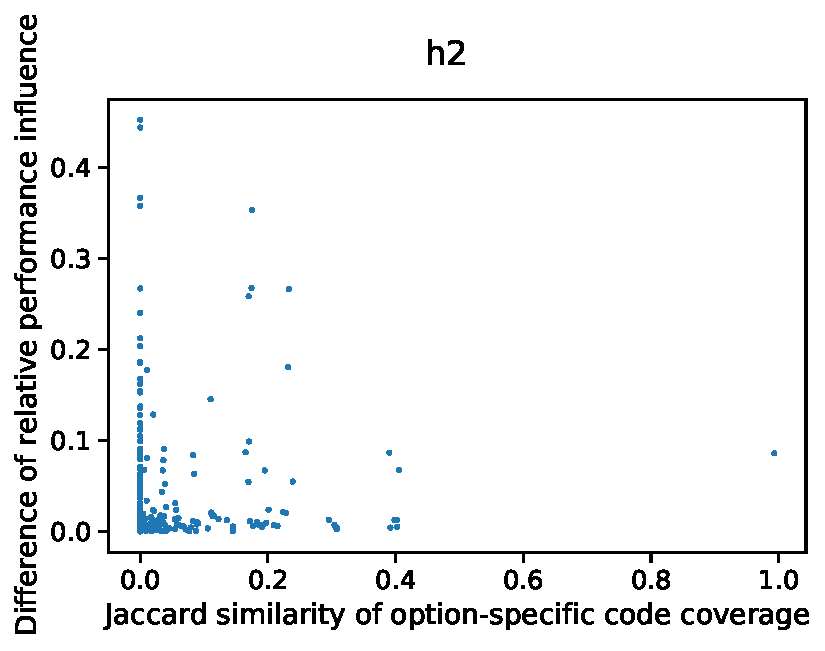
\includegraphics[width=\linewidth]{images/rq3.2/h2_rq3.2.pdf}
		%\caption{\htwo}
	\end{subfigure}
	\begin{subfigure}{0.33\textwidth}
		\centering
		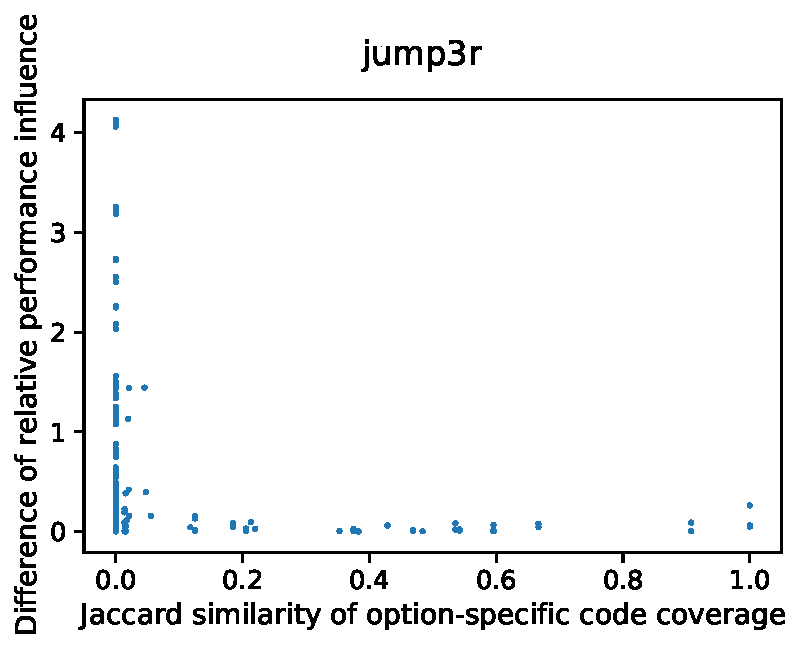
\includegraphics[width=\linewidth]{images/rq3.2/jump3r_rq3.2.pdf}
		%\caption{\jumper}
	\end{subfigure}
	\begin{subfigure}{0.33\textwidth}
		\centering
		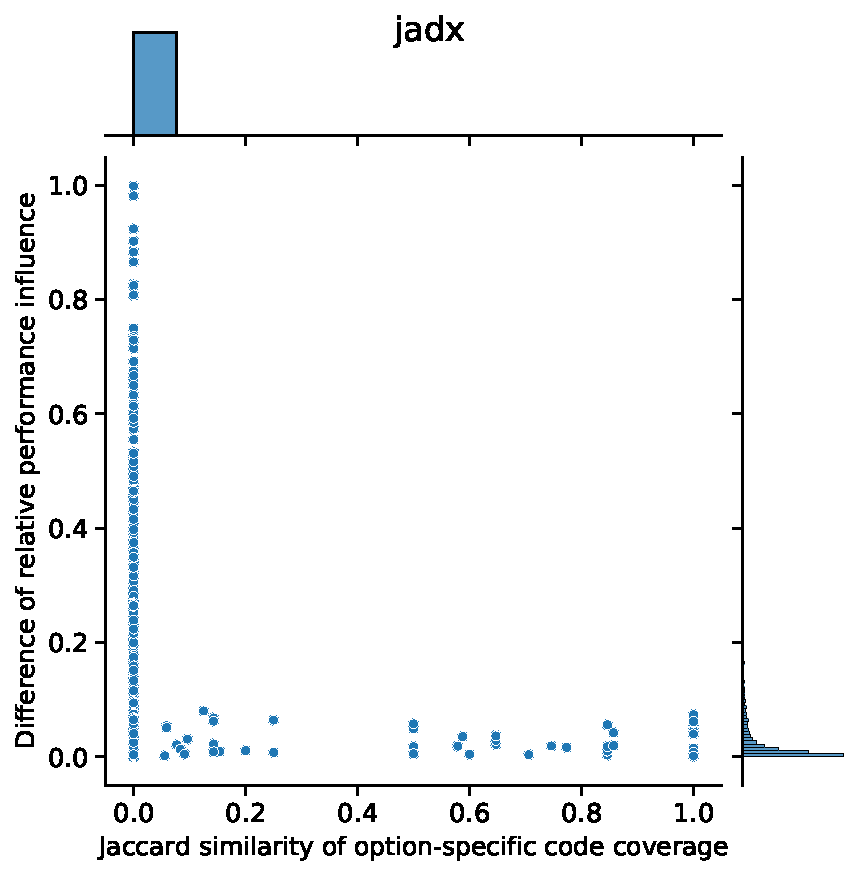
\includegraphics[width=\linewidth]{images/rq3.2/jadx_rq3.2.pdf}
		%\caption{\jadx}
	\end{subfigure}
	\begin{subfigure}{0.33\textwidth}
		\centering
		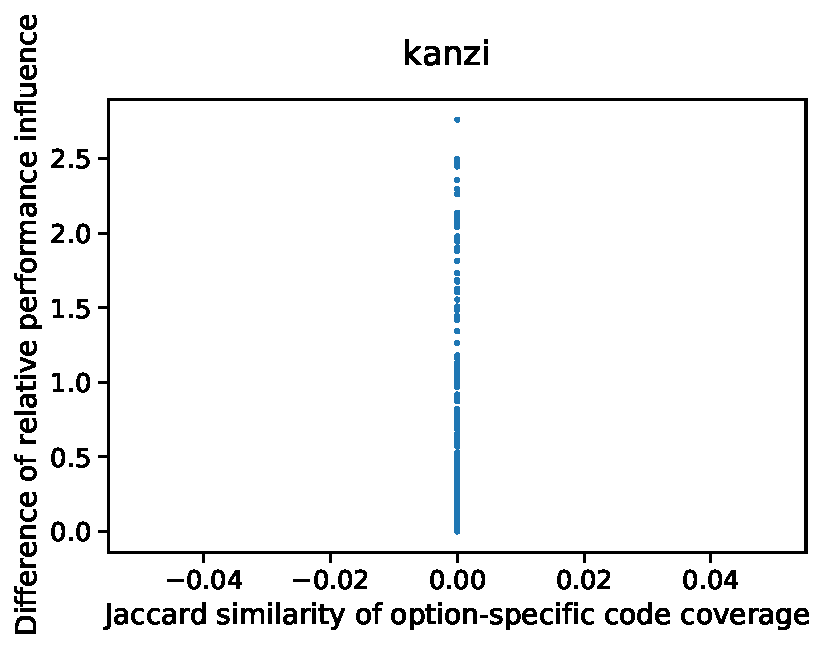
\includegraphics[width=\linewidth]{images/rq3.2/kanzi_rq3.2.pdf}
		%\caption{\kanzi}
	\end{subfigure}
	\caption{Differences in performance influence/importance vs. differences in option code coverage.}
	\label{fig:diff_performance_option_coverage}
\end{figure*}

\section{Discussion}
The results from our evaluation make a case for incorporating workload characteristics as independent variables into the analysis of the performance of configurable software systems. We discuss this facet in detail in the following and set the results into the context of transfer learning for performance models and give an outlook on methodologies to capture workload-specific performance variation.

\subsection{Workload-aware Performance Models}
In \RQref{3}, we observed that, except for \jadx, the workload-specific code usage is the most plausible cause for workload-specific variation of configuration options’ performance influence. Thus, we conclude that it is more decisive for the performance of a software system in general, \emph{how} different workloads use covered code, and not necessarily, \emph{what} code is covered. Our results confirm the prevalence of interactions between workload and configuration options as illustrated in our introductory example in Figure~\ref{fig:intro}. While this particular example and the majority of cases in this study are rather one-dimensional as they scale with the workload size (for instance, the number of transactions or the file size), the fact that we also found configuration options only becoming influential at all under a specific workload (\kanzi and \dconvert), highlights that one cannot assume such straightforward behavior in every case. 

To make these findings useful in practice, it is key to understand which \emph{qualitative} (e.g., file type or transaction type) and \emph{quantitative} (e.g., file size or number query length) workload properties interact with different configuration options and how. In the field of performance testing, assessing workload characteristics is already established practice to select workloads that are representative of usage patterns in production. Our results provide an empirical motivation to expand the use of \emph{workload characterization} as an engineering practice~\cite{calzarossa2016} to systematically test the sensitivity of configuration options to workload characteristics. To obtain representative performance models, they need to reflect the performance variation that different workloads can introduce.

\subsection{Implications for Transfer Learning}
The results from \RQref{1} and \RQref{2} illustrate that, even among a small number of configurable software systems, the configuration-specific performance behavior across workloads as well as the number of option-specific performance influences affected by the workload can vary widely. The substantial number of performance distributions classified as dissimilar is potentially challenging for transfer learning approaches that aim at adapting workload-specific performance models to new
workloads. 

Approaches like the work by \citeauthor{jamshidi_learning_2018} exploit similarities between workload-specific performance distributions~\cite{jamshidi_learning_2018}, such as scenarios in which the option influences are shifted by a constant amount or scaled by a factor proportional to the workload size (cf. Figure ~\ref{fig:intro}). While these are relatively simple scenarios that are accountable to affine transformations and more complex non-linear relationships could be learned, our results do not suggest that transfer learning is an economical or feasible option to handle differences in workload-specific performance behavior in
every case. Given the prevalence of different degrees of variation (cf. Table~\ref{tab:categorization}), one cannot assume that a configurable software system
and workload pair provides exploitable similarities, so that learning a new workload-specific performance model or workload-aware performance model from scratch may be the better choice in the long run.

\subsection{Capturing Workload-specific Performance Variation}
In our experiments, we used statement coverage as a proxy metric to describe \emph{what} option-specific code is executed, but cannot make statements about \emph{how} a workload exercised the covered code. We can infer only that variation in the latter most likely accounts for workload-specific performance variation. Aside from incorporating workload characteristics as features in a workload-aware performance model, performance measurement at a finer granularity, such as method or statement level, is a methodology that might be beneficial to our analysis. Work closest to such a methodology is the white-box profiling approach by \citeauthor{weber_white_2021}~\cite{weber_white_2021}. They use a fine-grained profiler to assess at method level which factors, either configuration options or application context (e.g., method arguments), account for a method's performance. 

In the light of our findings from \RQref{3}, we believe that fine-grained performance measurements are a worthwhile strategy to identify code sections whose performance is influenced by the workload and options in concert.

\section{Threats to Validity}\label{sec:threats}

\paragraph*{Internal Validity}\label{sec:internal_validity}
Threats to \emph{internal validity} include measurement noise which may distort our classification into categories (Section~\ref{sec:rq1}) and model construction (Section~\ref{sec:rq2}). We mitigate this threat by repeating each experiment five times and reporting the median as a robust measure. For \htwo, we confirmed a negligible measurement variation in a separate pre-study.
Another potential threat is that the coverage analysis with \mbox{\textsc{JaCoCo}} entails a noticeable instrumentation overhead, which may distort performance observations. We mitigate this threat by separating the experiment runs for coverage assessment and performance measurement. In the case of \htwo, the load generator of the \textsc{OLTPBench} framework~\cite{difallah_oltp_2013} ran on the same machine as the database since we were testing an embedded scenario but thus introduced only negligible variation and overhead.

\paragraph*{External Validity}\label{sec:external_validity}
The selection of subject systems all written in Java poses a threat to \emph{external validity}. While our motivation for this selection is primarily practical (cf. Section~\ref{sec:setup}), we mitigate this threat by selecting subject systems from a variety of application domains (cf.~Table~\ref{tab:subject_systems}). Nonetheless, one cannot necessarily conclude that our results hold for other domains and programming languages. 

\paragraph*{Construct Validity}\label{sec:construct_validity}
The profiler \textsc{JaCoCo} instruments Java byte code instructions rather than statements, which leads to some minor imprecision when mapping covered instructions back to the original statements. Transitively, this also affects the precision of our feature location (cf. Section~\ref{sec:rq3}). This drawback, however, is not limited to this particular profiler but applies to most profilers operating on byte code. 
Superimposition in our feature location technique is sound, but, by design, incomplete, since no set of workloads is guaranteed to cover all feature code. We selected a variety of different workloads as a countermeasure, yet our study is exploratory. 

{\color{blue}
\section{Conclusion}
Software performance emerges from a multitude of factors. Configuration options have been widely studied as a key factor and used for learning performance models.  When learning configuration-dependent performance models, workloads as an orthogonal factor have so far been overlooked---most approaches rely on performance observations using a single workload. This raises the question of how generalizable existing models are to other workloads. 
Understanding to what extent configuration and workload---individually and combined---are responsible for the performance variation of a software system is key to evaluate whether one can transfer existing performance models to new workloads, or has to learn performance models from scratch for new workloads.

In an empirical study of 29\,014 configurations and 55 workloads, we explore both sides: how varying the workload affects the performance behavior and execution across the configuration space of 6 configurable software systems. Specifically, we investigate (1) whether the workload and configuration interact and in conjunction influence performance and, if so, (2) how this interaction takes place.
We enrich our black-box performance observations with statement coverage data to understand performance variation, and especially the corresponding execution, at a fine granularity.
Our findings suggest that the workload-specific execution of visited option-specific code segments plays a substantial role in how workloads interact with configurations and is most likely accountable for workload-specific performance variation. 
We conclude that identifying performance-relevant workload characteristics and incorporating them as independent variables is a promising avenue towards obtaining generalizable and representative performance models.
The wide variety of workload-specific effects on performance that we observe can challenge the feasibility of existing transfer learning approaches for performance models. In essence, one cannot assume that an existing  workload-specific performance model is easily transferable to a new workload with little effort. While transfer learning can capture the majority of workload-specific differences in performance influences, we conclude that, at large, workload-aware performance models may be a better choice.

In further work, we will incorporate workload characteristics as well as further factors of variation, such as hardware variability and the evolution of configurable software systems, into our analysis.

}
	
	
	\clearpage
	\bibliographystyle{ACM-Reference-Format}
	\bibliography{literature}
\end{document}
\endinput
%%
%% End of file `sample-sigconf.tex'.
